\subsection{RQ1: Generated CSA Checkers}

Table~\ref{tab:all39-system} reports all 39 subjects and the preexisting 15-case noisy stratum. Zero starting PDS is an entry condition, not KNighter's refinement result. Every portfolio retains the 15 initially warning-positive vulnerable revisions. Among the 24 initially silent subjects, native recovers 8, no-internal 6, and KNighter 0 under its actual no-report policy. These are warning signals, not verified target-recall counts.

\begin{table}[!htbp]
\centering
\caption{CSA comparison: (a) all 39 subjects; (b) the complete preexisting 15-case fixed-noisy stratum, reusing the same outputs. TP/FP/FN are version-warning decisions; fixed reports measure burden and replies count received responses. Color shades $1-F_1$ at .25/.50/.75, not significance.}
\label{tab:all39-system}
\label{tab:matched14}
\begingroup\FTTableSetup
\begin{tabular}{l|cccc|c|cc}
\multicolumn{8}{l}{(a) Full cohort: 39 subjects}\\
\hline\hline
\multirow{2}{*}{Condition}&\multicolumn{4}{c|}{Version outcomes}&
\multirow{2}{*}{$F_1$}&\multicolumn{2}{c}{Burden / effort}\\
\cline{2-5}\cline{7-8}
&PDS&TP&FP&FN&&Fixed reports&Replies\\\hline
Unmodified &0&15&15&24&\FTFScore{.435}&73&0\\\hline
KNighter loop &2&15&13&24&\FTFScore{.448}&69&179\\\hline
\toolname, native &5&23&18&16&\FTFScore{.5750}&123&150\\\hline
\toolname, no internal &8&21&13&18&\FTFScore{.5753}&68&133\\
\hline\hline
\end{tabular}
\par\smallskip
\begin{tabular}{l|c|c|c}
\multicolumn{4}{l}{(b) Noisy 15: all methods retain TP=15, PDS=2 and $F_1=.6977$}\\
\hline\hline
& KNighter loop & Native & No internal\\\hline
Fixed reports &69&44&68\\
\hline\hline
\end{tabular}
\endgroup
\end{table}

Warning coverage and report burden move in different directions: native's 123 fixed reports exceed no-internal's 68 and KNighter's 69; its precision is $0.561$ versus $0.618$ for no-internal. The nearly tied $F_1$ summarizes different coverage/noise portfolios and does not establish native superiority. G12 contributes 73 distinct fixed-side warning locations, not duplicates; its broader matching yields 74 vulnerable and 73 fixed reports. This unfavorable tradeoff remains in the aggregate.

In the complete 15-case fixed-noisy stratum (Table~\ref{tab:matched14}b), native reduces reports by 25 (36.2\%) against KNighter and 24 (35.3\%) against control. The effect is concentrated in G24's $27\rightarrow2$ fixed reports; other small differences offset one another. Identical binary fixed positivity and $F_1$ thus coexist with different report burdens. The follow-up finds G24's retained reports outside the target lifecycle (Section~\ref{sec:target-results}); the lower count is therefore not evidence of target-preserving suppression.

\subsection{RQ2: Cross-Backend Feasibility}

A separate archived automatic ImageMagick CodeQL query starts at $0/0$ vulnerable/fixed rows. Table~\ref{tab:codeql-decoding} includes two $8/0$ recoveries and the third decode's $22/22$ outcome. The successful edit corrects relative-path matching while keeping exact file/function/local-variable filters. This demonstrates patch-local operation on a second format, not broad backend transfer or native-evidence causality. A second query already starts at $2/0$ and is not counted as a gain. KNighter is not a CodeQL baseline.

\begin{table}[!htbp]
\centering
\caption{Three automatic CodeQL decodes of one query. Counts are vulnerable/fixed output rows; time is recorded agent-round duration, excluding separate paired replay.}
\label{tab:codeql-decoding}
\begingroup\FTTableSetup
\begin{tabular}{c|c|crr}
\hline\hline
Decode & V/F rows & Replies & Tokens & Agent time (s)\\\hline
1 &8/0&1&15,122&87.87\\
2 &8/0&1&14,345&42.74\\
3 &22/22&8&110,282&516.77\\
\hline\hline
\end{tabular}\endgroup
\end{table}

\textbf{Second-backend costs.} Table~\ref{tab:codeql-decoding} reports the original model runs. Three warm paired replays per query preserve $0/0$ and $8/0$. Median query-plus-decode time is 12.57\,s initially and 36.51\,s after refinement with two threads; peak process RSS is 976/1,078\,MiB. Database-creation log intervals span 31/30\,s, excluding unlogged startup. Developer labor is unmeasured. These one-case existing-environment observations are neither a speedup, cold-install benchmark nor whole-project scalability estimate.

\subsection{RQ3: Internal-Evidence Sensitivity}

Table~\ref{tab:origin-types} reports initial record provenance; Section~\ref{sec:evidence-roles} defines native types and source-derived context. Dynamic availability has a separate denominator: 103 of 150 unique native-chain attempts have usable hash-bound observations; 11 are unavailable due to candidate compilation, 18 unsupported context, 13 zero scoped callbacks, 1 reproduced candidate crash and 4 capped optional observations. None establishes safety from absence.

Across 39 subjects, native has six comparative benefits, five disadvantages and 28 ties/other outcomes. The associated edits expose concrete differences in checker behavior: cleanup-wrapper recognition in G19, nested dereference/binding recovery in G25, and null/region/frame handling in G24. G19 adds \texttt{\_\_free\_kfree} to a cleanup predicate, yielding $15/0$ versus control's $0/0$; 15 reports are not 15 bugs. Conversely, control recovers symbolic-region handling in G23 and persistent-field release recognition in G38 without native records. G12 drops CPU-role restrictions, explaining its broad matching and noise. These code observations distinguish repairs from broader matching; a record's presence or an LLM explanation alone does not prove edit causality.

\begin{figure}[!htbp]
\centering
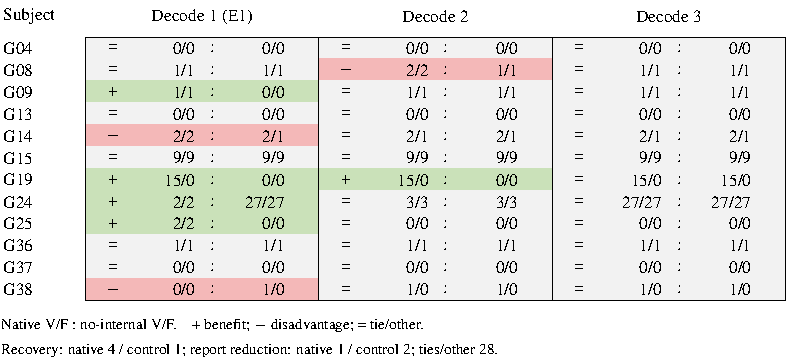
\includegraphics[width=378bp]{figures/fig-e3-repeats.pdf}
\Description{A twelve-subject by three-decode matrix of native and no-internal vulnerable/fixed warning counts, highlighting comparative benefits, disadvantages and ties.}
\caption{E3: all 36 paired decodes on 12 subjects; cells compare native and no-internal V/F counts. Decode 1 reuses E1; the remaining decodes add 48 condition cells. Color and sign encode the comparative direction.}
\label{fig:repeats}
\end{figure}

Figure~\ref{fig:repeats} shows five subjects tying in all three decodes and seven with mixed directions; none benefits comparatively in all three. G19's native $15/0$ recurs, but control catches up in its third decode. G24's main reduction does not repeat. G14's $3/3\rightarrow2/2$ improves its own start but trails control's $2/1$; later decodes tie. In the main comparison, G05/G23/G38 retain initially $0/0$ in native while control recovers warnings, so their disadvantage is not loss of an initial signal. Repeated subjects, selection/reuse and native-only gating limit stronger attribution. Realized call differences under a shared stopping rule are outcomes/mediators, not independently assigned confounds.

\subsection{RQ4: Model Configuration Sensitivity}

Table~\ref{tab:models39} uses the original 12 subjects, native only, one decode per model, 2-reply and 65,536-output ceilings with requested high effort. All configurations retain the five initial vulnerable warning signals and recover additional versions. Flash has the strongest observed outcome here, but one decode on this subset does not establish general ranking or variance-controlled model robustness.

\begin{table}[!htbp]
\centering
\caption{Limited-budget native sensitivity: 12 subjects per model, not full-39 robustness. Computation differs despite common reply/output ceilings. $F_1$ shading follows Table~\ref{tab:all39-system}.}
\label{tab:models39}
\begingroup\FTTableSetup
\begin{tabular}{l|ccc|c|cc}
\hline\hline
Editor & TP & FP & PDS & $F_1$ & Fixed reports & Replies\\
\hline
Unmodified &5&5&0&\FTFScore{.455}&42&0\\\hline
GPT-6-Luna high &7&6&1&\FTFScore{.560}&40&24\\\hline
GLM-5.3 high &7&5&2&\FTFScore{.583}&16&23\\\hline
GLM-5.3-Flash high &9&5&4&\FTFScore{.692}&11&21\\
\hline\hline
\end{tabular}
\endgroup
\end{table}

Received replies total 24/23/21 respectively. Capped, format-invalid and compile-failed replies remain charged; a healthy previous detector is retained when no valid improvement occurs. These are complete workflow outcomes, not successful code generation on every call. No no-internal arm is run across models, so E4 cannot isolate cross-model evidence effects.

\subsection{What the Observed Improvements Establish}
\label{sec:target-results}

\textbf{Complete non-tie audit.} Of the six warning-based native benefits, G12/G19/G25 have bounded source-supported target reports; G09 has conditional support; G24/G35 have no supported or conditional retained target report. Of the five control advantages, G01/G23/G38 have bounded source-supported target reports and G05/G14 have conditional support. These describe the complete selected subset, not corrected success rates or independently adjudicated target accuracy.

The code changes explain why these categories differ. Both G01 arms recover the governing loop, but only control adds a capacity/break guard; native's fixed reports contradict the actual guard. G19 adds a lowered cleanup name, while G23 control recovers symbolic-region and nested-member handling. G25's native changes add nested sink recognition and destination binding. Recognition therefore improves in both arms, but is separate from guard and state correctness. G05 preserves uncertain initialization; G09 broadens cleanup handling; G12 removes actor restrictions; G35 broadens status/condition reporting. Their recovered reports range from conditional target concerns to unrelated, contradicted reports. G38 control preserves field identity while relaxing a usage gate, with bounded reference-lifetime support.

Report reduction can also change the surviving report population. G14's arms project onto different completion/free events; one fixed control report concerns a different supported stack-lifetime risk. G24 removes 25 reports per side, but its two retained native reports concern destroyed owners rather than the intended surviving-owner lifecycle. This does not prove loss of a previously valid witness; it does show that nonzero vulnerable warning presence cannot certify target preservation.

\textbf{Frozen perturbations.} Each primary mechanism has six positive and six negative fixtures. G12 reports at a target location in all positive fixtures and none of the negative ones, within its annotation model; its remote-write note still points to a local reset. G19 is silent on its adapted-wrapper suite. Its separate canonical control yields one supported early-exit report plus a wrong-scope allocator-return report, and misses the renamed wrapper. G25 has target-location reports in all six positive and five negative fixtures. Starting/control artifacts are silent for these three cases. In G24, starting/control has target-location reports in all six positive and six negative fixtures with 108/108 total reports; native has none with 18/12 total reports, although secondary review supports guard warnings outside the frozen target-line list. These disagreements remain visible rather than changing the scoring rule after inspection.

\textbf{Selected-clue intervention.} All three full G25 decisions peel outer sink-expression casts; no withheld decision does. Two full decisions also change bookkeeping. Table~\ref{tab:checkpoint-intervention} reports the separate compiler-completed artifacts: full recovers target-line presence with negative-side noise, while withheld remains silent. This rules out uncompiled controls as the sole reason for terminal silence, but does not establish three valid detection gains: all 34 reports from full repetitions 2/3 take \texttt{argc<=1}, which selects a concrete non-NULL object. Full repetition 1 has six outer count-access reports admitting a source-feasible NULL completion, without an explicit NULL-return event, alongside unsupported reports.

\begin{table}[!htbp]
\centering
\caption{GLM-5.3-Flash bounded-adapter terminal artifacts after separate compiler-only completion. Each cell is full/withheld. Primary suites have six positive and six negative fixtures; G19 lowering has two of each and benign has four negatives. Hits/alerts are final-location presence, not validated diagnoses. Original strict/adapter failures remain separate (Section~\ref{sec:target-followup}).}
\label{tab:checkpoint-intervention}
\begingroup\FTTableSetup
\begin{tabular}{c|ccc|ccc}
\hline\hline
\multirow{2}{*}{Draw}&\multicolumn{3}{c|}{G19}&\multicolumn{3}{c}{G25}\\
\cline{2-7}
&\shortstack{Primary\\positive hits}&\shortstack{Lowering\\positive hits}&\shortstack{Benign\\alerts}&\shortstack{Positive\\hits}&\shortstack{Negative\\alerts}&\shortstack{Negative\\reports}\\\hline
1&0/6&1/2&0/2&6/0&5/0&28/0\\
2&0/6&1/2&0/2&6/0&5/0&10/0\\
3&6/0&2/0&1/0&6/0&6/0&6/0\\
\hline\hline
\end{tabular}\endgroup
\end{table}

G19 instead exposes a coverage/noise tradeoff. Full repetitions 1/2 retain name-family tests; withheld generalizes registration, while repetition 3 reverses primary coverage. The broader matchers can warn on benign cleanup. Across the reviewed G19 artifacts, supported owning-scope exits coexist with reports at callee returns and a write-only cleanup mistaken for a read. This is selected-checkpoint evidence, not a population effect or a rule predicting useful native context.

\textbf{Resulting engineering distinction.} The same source line can contain a safe pointer-field read and the actual optional-object dereference, while a relevant guard report can lie outside a frozen sink-line list. Thus neither report presence nor final-line association substitutes for the reported object, operation, path and owning scope. The contribution is the evidence-linked explanation of these divergences; the source judgments remain bounded and do not turn the workflow into a semantic verifier.
